\section{Zombieland II}
\subsection{Descripci\'on de la problem\'atica}
\subsection{Resoluci\'on propuesta y justificaci\'on}
\subsection{An\'alisis de la complejidad}

\newpage

\subsection{C\'odigo fuente}
	\begin{codesnippet}
	\begin{verbatim}
    struct posYsold {
        int soldadosVivos;
        int i;
        int j;
    };
	\end{verbatim}
	\end{codesnippet}

	\begin{codesnippet}
	\begin{verbatim}
    Matriz ciudadInfestada;
    unsigned int n, m;
    
    int main(int argc, char const *argv[]){
        unsigned int s;
        cin >> n >> m >> s;
        unsigned int inicioH, inicioV, bunkerH, bunkerV;
        cin >> inicioH >> inicioV >> bunkerH >> bunkerV;
        inicioV--;
        inicioH--;
        bunkerV--;
        bunkerH--;
    //la matriz de la ciudad guarda cuantos zombies tiene el eje para moverse
    // a la derecha y hacia abajo (en ese orden)
    //para la izquierda es ir al de la izquierda y preguntar por el derecho
    //para arriba es ir al de arriba y preguntar por el de abajo
        ciudadInfestada = Matriz(n, vector<pair<int, int> >(m));
        for (int i = 0; i < n-1; ++i) {
            for (int j = 0; j < m-1; ++j) {
                cin >> ciudadInfestada[i][j].first;
            }
    //no hay camino a la derecha
            ciudadInfestada[i][m-1].first = -1;
            for (int j = 0; j < m; ++j) {
                cin >> ciudadInfestada[i][j].second;
            }
        }
        for (int j = 0; j < m-1; ++j) {
            cin >> ciudadInfestada[n-1][j].first;
    //no hay camino hacia abajo
            ciudadInfestada[n-1][j].second = -1;
        }
    //no hay camino a la derecha ni abajo
        ciudadInfestada[n-1][m-1].first = -1;
        ciudadInfestada[n-1][m-1].second = -1;
    //creamos el cubo a completar
        Cubo grafo(n, vector<vector<pair<posYsold, bool> > >(m));
        for (int i = 0; i < n; ++i) {
            for (int j = 0; j < m; ++j) {
                grafo[i][j] = vector<pair<posYsold, bool> >(s+1);
            }
        }
    //aplicamos el algoritmo
        int soldadosVivos = zombieland(grafo, inicioH, inicioV, bunkerH, bunkerV, s);
	\end{verbatim}
	\end{codesnippet}

	\begin{codesnippet}
	\begin{verbatim}
    //cout pedido
        cout << soldadosVivos << endl;
        deque<posYsold> recorrido;
    //para armarlo desde el principio hasta el final
        if(soldadosVivos != 0){
            posYsold posActual;
            posActual.soldadosVivos = soldadosVivos;
            posActual.i = bunkerH;
            posActual.j = bunkerV;
            while(posActual.i != inicioH || posActual.j != inicioV){
                recorrido.push_front(posActual);
                posActual = grafo[posActual.i][posActual.j][posActual.soldadosVivos].first;
            }
            posActual.soldadosVivos = s;
            posActual.i = inicioH;
            posActual.j = inicioV;
            recorrido.push_front(posActual);
        }
        for (int i = 0; i < recorrido.size(); ++i) {
            cout << recorrido[i].i+1 << " " << recorrido[i].j+1 << endl;
        }
        return 0;
    }
	\end{verbatim}
	\end{codesnippet}

	\begin{codesnippet}
	\begin{verbatim}
    int zombieland(Cubo& grafo, int inicioH, int inicioV, int bunkerH, int bunkerV, int soldados){
        int maxSoldados = 0;
    //cola para el BFS arranca con la posicion de donde salimos
        queue<posYsold> cola;
        posYsold actual;
        actual.soldadosVivos = soldados;
        actual.i = inicioH;
        actual.j = inicioV;
        cola.push(actual);
    //se marca esta posicion como visitada
        grafo[inicioH][inicioV][soldados].second = true;
        int zombies;
        int resultadoBatalla;
    //mientras tengamos algo para visitar (no sabemos si llegaremos al final)
        while(cola.size() > 0){
    //actual es el primero de la cola
            actual = cola.front();
        //si no estamos el final vemos si podemos ir a cada una de las cuatro direcciones
        //si es valido, no se mueren todos los soldados y no visite ese nodo, 
        //agregare el siguiente nodo a visitar
        //si ya lo visite, existe un camino que me lleva hasta ahi, 
        //ya fue encolado el camino que le sigue
            if(!(actual.i == bunkerH && actual.j == bunkerV)){
                zombies = zombiesCuadra(actual.i, actual.j, ARRIBA);
                resultadoBatalla = resulBatalla(actual.soldadosVivos, zombies);
                if(zombies != -1 && resultadoBatalla > 0 && !grafo[actual.i-1][actual.j]
                [resultadoBatalla].second){
                    posYsold arriba;
                    arriba.soldadosVivos = resultadoBatalla;
                    arriba.i = actual.i-1;
                    arriba.j = actual.j;
                    cola.push(arriba);
                    grafo[actual.i-1][actual.j][resultadoBatalla].second = true;
                    grafo[actual.i-1][actual.j][resultadoBatalla].first = actual;
                }
                zombies = zombiesCuadra(actual.i, actual.j, DER);
                resultadoBatalla = resulBatalla(actual.soldadosVivos, zombies);
                if(zombies != -1 && resultadoBatalla > 0 && !grafo[actual.i][actual.j+1]
                [resultadoBatalla].second){
                    posYsold der;
                    der.soldadosVivos = resultadoBatalla;
                    der.i = actual.i;
                    der.j = actual.j+1;
                    cola.push(der);
                    grafo[actual.i][actual.j+1][resultadoBatalla].second = true;
                    grafo[actual.i][actual.j+1][resultadoBatalla].first = actual;
                }
	\end{verbatim}
	\end{codesnippet}

	\begin{codesnippet}
	\begin{verbatim}
                zombies = zombiesCuadra(actual.i, actual.j, ABAJO);
                resultadoBatalla = resulBatalla(actual.soldadosVivos, zombies);
                if(zombies != -1 && resultadoBatalla > 0 && !grafo[actual.i+1][actual.j]
                [resultadoBatalla].second){
                    posYsold abajo;
                    abajo.soldadosVivos = resultadoBatalla;
                    abajo.i = actual.i+1;
                    abajo.j = actual.j;
                    cola.push(abajo);
                    grafo[actual.i+1][actual.j][resultadoBatalla].second = true;
                    grafo[actual.i+1][actual.j][resultadoBatalla].first = actual;
                }
                zombies = zombiesCuadra(actual.i, actual.j, IZQ);
                resultadoBatalla = resulBatalla(actual.soldadosVivos, zombies);
                if(zombies != -1 && resultadoBatalla > 0 && !grafo[actual.i][actual.j-1]
                [resultadoBatalla].second){
                    posYsold izq;
                    izq.soldadosVivos = resultadoBatalla;
                    izq.i = actual.i;
                    izq.j = actual.j-1;
                    cola.push(izq);
                    grafo[actual.i][actual.j-1][resultadoBatalla].second = true;
                    grafo[actual.i][actual.j-1][resultadoBatalla].first = actual;
                }
            }
        //si llegamos al final, actualizamos los soldados que quedaron vivos, 
        //si es mayor a haber llegado por otro camino
            else
                if(maxSoldados < actual.soldadosVivos)
                    maxSoldados = actual.soldadosVivos;
        //desencolo el nodo que estaba analizando
            cola.pop();
        }
        return maxSoldados;
    }
	\end{verbatim}
	\end{codesnippet}

	\begin{codesnippet}
	\begin{verbatim}
    int zombiesCuadra(int i, int j, movimiento mov){
    //devuelve los zombies que en la cuadra pedida
        switch(mov){
            case ARRIBA:
                if(i == 0)
                    return -1;
                return ciudadInfestada[i-1][j].second;
            case ABAJO:
                return ciudadInfestada[i][j].second;
            case IZQ:
                if(j == 0)
                    return -1;
                return ciudadInfestada[i][j-1].first;
            case DER:
                return ciudadInfestada[i][j].first;
        }
    }
	\end{verbatim}
	\end{codesnippet}

	\begin{codesnippet}
	\begin{verbatim}
    int resulBatalla(int sold, int zomb){
    //devuelve si es posible pasar por una cuadra
        if(sold>=zomb)
            return sold;
        return sold-(zomb-sold); 
    }
	\end{verbatim}
	\end{codesnippet}

\newpage

\subsection{Experimentaci\'on}
\subsubsection{Constrastaci\'on Emp\'irica de la complejidad}
Para realizar los experimentos, se consideró como peor caso, aquel en el que se debiera recorrer cada nodo de la ciudad, tantas veces como cantidad de soldados se tuviese a disposicion, siendo ese caso, en el que se recorrerían $s.n.m$ elementos, coiniciendo así con la complejidad teórica $O(s.n.m)$.\\
Aunque ese el caso deseable, generar dicha instancia para los distintos valores de $s$, $n$ y $m$, resultó tan dificultoso como resolver el problema en cuestión.\\
Por ello, se decidio generar instancias con una cantidad aleatoria de zombies por cuadra. Ésto permitió generar instancias automáticamente, para casos de prueba grandes, pero trajo consigo los siguientes problemas:
\begin{enumerate}
	\item No se puede determinar si existe un camino desde el punto de inicio hasta el búnker.
	\item No se puede determinar, si al existir un camino, este será único.
	\item No se puede determinar cuantos soldados van a llegar al búnker.
	\item No se puede determinar cuantos caminos adulteran la cantidad de soldados, ni cuantos soldados mueren en cada uno de ellos.
\end{enumerate}

El resultado del generador de instancias, proporcionaba un laberinto como el siguiente:

\begin{center}
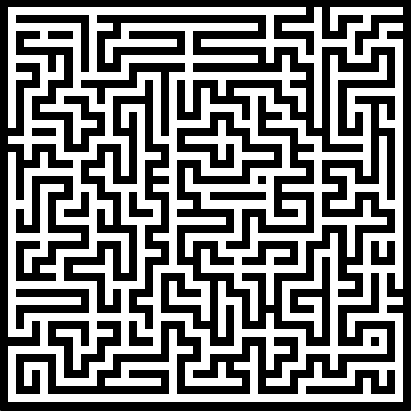
\includegraphics[width=7cm,keepaspectratio=yes]{imagenes/ej2/maze.png}
\end{center}

Los pasajes del laberinto son los caminos donde hay entre $0$ y $s+1$ zombies, y las paredes, caminos donde hay entre $0$ y $s$.2.\\
Estos valores aleatorios fueron tomados adrede, por un lado, para que incluso el mejor camino (alguno de los pasajes que conducen a la salida), tuviera perdida de soldados, pero intentando que éstas sean mínimas, para aumentar las probabilidades de que puedan efectivamente llegar al búnker.
Las paredes, no son un obstaculo, dado que podrían terminar siendo un pasaje, pero la probabilidad de que eso ocurra es muy baja.\\
Aún asi, el $s$ tomado en el algoritmo aleatorio es el que se recibe en la entrada. Esto significa, que se configura al principio, y despues no se actualiza con la cantidad de soldados despues de una batalla.\\
Por ende, no podemos determinar el porcentaje de soldados totales que llegarán, pero sí podemos saber el porcentaje que sobrevivirá a la primer batalla.\\
Así, la cantidad de soldados que sobreviviran a la primer batalla es:
\begin{itemize}
	\item 95\% en caso de que el camino sea un pasaje.
	\item 50\% en casos de que el camino sea una pared.
\end{itemize}
Estos rangos aleatorios también se obtuvieron experimentando, hasta lograr valores que ocasionaran bajas pero que no impidieran a los soldados llegar al búnker en la mayoría de los casos. Dichos experimentos exceden el interés de esta sección y no serán discutidos.\\

Pese a dificultades expuestas, se decidió proceder con dichas instancias, ya que lograban generar una fluctuación en la cantidad de soldados, y esto, si bien lejos del peor caso propuesto, resultó ser una aproximación que nos resultó suficiente.\\

Por lo dicho anteriormente, se realizaron experimentos sobre los siguientes dos casos:
\begin{itemize}
	\item \textbf{Cero zombies}: En esta instancia, la cantidad de zombies en cada cuadra es cero, con lo cual, el algoritmo recorre toda la ciudad, y se queda con cualquier camino.
	\item \textbf{Zombies aleatorios}: Es la instancia explicada anteriormente.
\end{itemize}

También es necesario aclarar, que los experimentos se realizaron sobre ciudades cuadradas, con puntos de inicio y llegada en los extremos opuestos de la ciudad, y con cantidad de soldados iniciales igual a 20.\\

A continuación se detallan los experimentos y sus resultados.
Debido al tamaño de las instancias de prueba, los inputs de dichos experimentos no fueron adjuntados.
\begin{center}
	\begin{tabular}{|c|c|c|}
	\hline
	Experimento & \textbf{Cero zombies} & \textbf{Zombies aleatorios}\\
	\hline
	\hline
	Tamaño de la ciudad & \multicolumn{2}{|c|}{Soldados al final}\\
	\hline
	50x50 & 20 & 6\\
	\hline
	100x100 & 20 & 19\\
	\hline
	250x250 & 20 & 17\\
	\hline
	500x500 & 20 & 17\\
	\hline
	750x750 & 20 & 16\\
	\hline
	1000x1000 & 20 & 12\\
	\hline
	1250x1250 & 20 & 20\\
	\hline
	1500x1500 & 20 & 7\\
	\hline
	1750x1750 & 20 & 14\\
	\hline
	2000x2000 & 20 & 20\\
	\hline
	\end{tabular}
\end{center}

Dado que los tiempos de ejecución para ambos experimentos varían ampliamente, primero analizaremos el experimento de \textbf{Cero zombies}.

\includegraphics[width=15cm,keepaspectratio=yes]{imagenes/ej2/czneto.png}

Como se puede apreciar, al no haber zombies, no existe ningun camino en el cual mueran soldados, por lo que los tiempos se incrementan acorde a la dimension de la ciudad, y al ser cuadradas, crece polinomialmente.

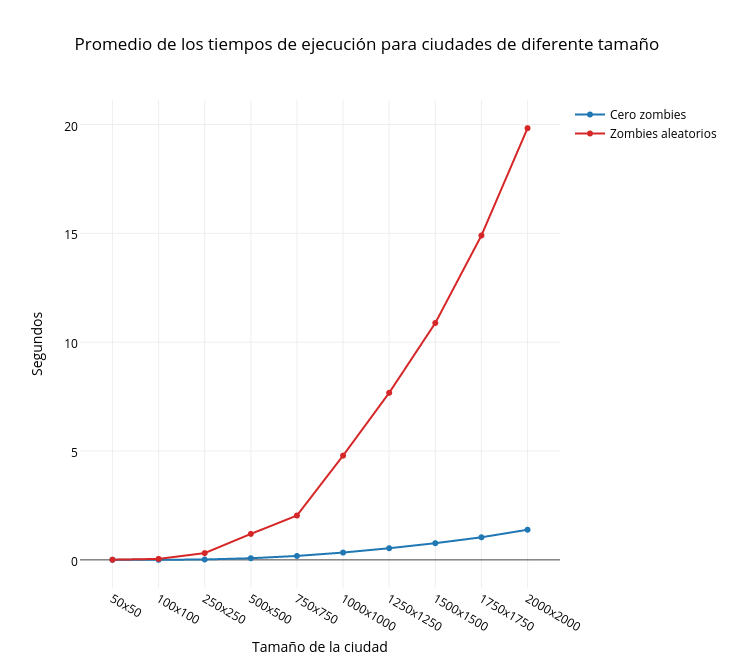
\includegraphics[width=15cm,keepaspectratio=yes]{imagenes/ej2/czyza.png}

Aquí se pueden apreciar las diferencias de tiempos. Ésta radica en el hecho de que \textbf{Zombies aleatorios} posee caminos en los cuales los soldados mueren. Por ello, el algoritmo deberá recorrer, en peor caso, $s$ veces la ciudad entera.\\

Se procedió, entonces, a dividir los resultados de \textbf{Zombies aleatorios} por la cantidad de soldados iniciales con los que se ejecutó el algoritmo a fin de que quede reflejado, que en ese caso, los tiempos serán muy similares a los de \textbf{Cero zombies}. Esto se debe a que ya no son los tiempos de recorrer $s$ veces la ciudad, sino de recorrerla una sola vez.
Sin embargo, es necesario aclarar que la similitud que se intenta mostrar, es aproximada, ya que no podemos asegurar que efectivamente, el algoritmo recorre $s$ veces la ciudad. Tal es el peor caso, y como hemos expuesto en un principio, no podemos asegurar que sea el que realmente ocurre.

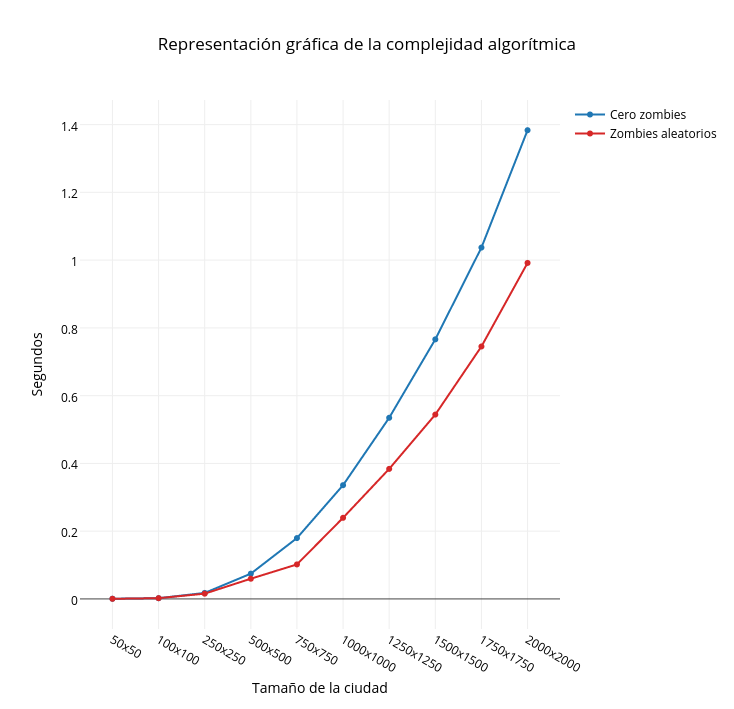
\includegraphics[width=15cm,keepaspectratio=yes]{imagenes/ej2/zaczados.png}

Manteniendo los resultados de \textbf{Zombies aleatorios} divididos por $s$, finalmente dividimos los resultados tanto de \textbf{Cero zombies} como de \textbf{Zombies aleatorios}, por $n$, y en una instancia aparte, por $n.m$.
De esta manera, dado que en ambos tienen $s$ igual a 1, solo queda ver que al dividir por $n$, los resultados se aproximan a una función lineal, y que al dividirlos por $n.m$, se aproximan a una constante.\\

Como solo nos interesa la relación, y no la función exacta ni la constante, multiplicamos los resultados de dichas divisiones por 100, para que los valores sean más claros y visibles.

\includegraphics[width=15cm,keepaspectratio=yes]{imagenes/ej2/linealizacion.png}

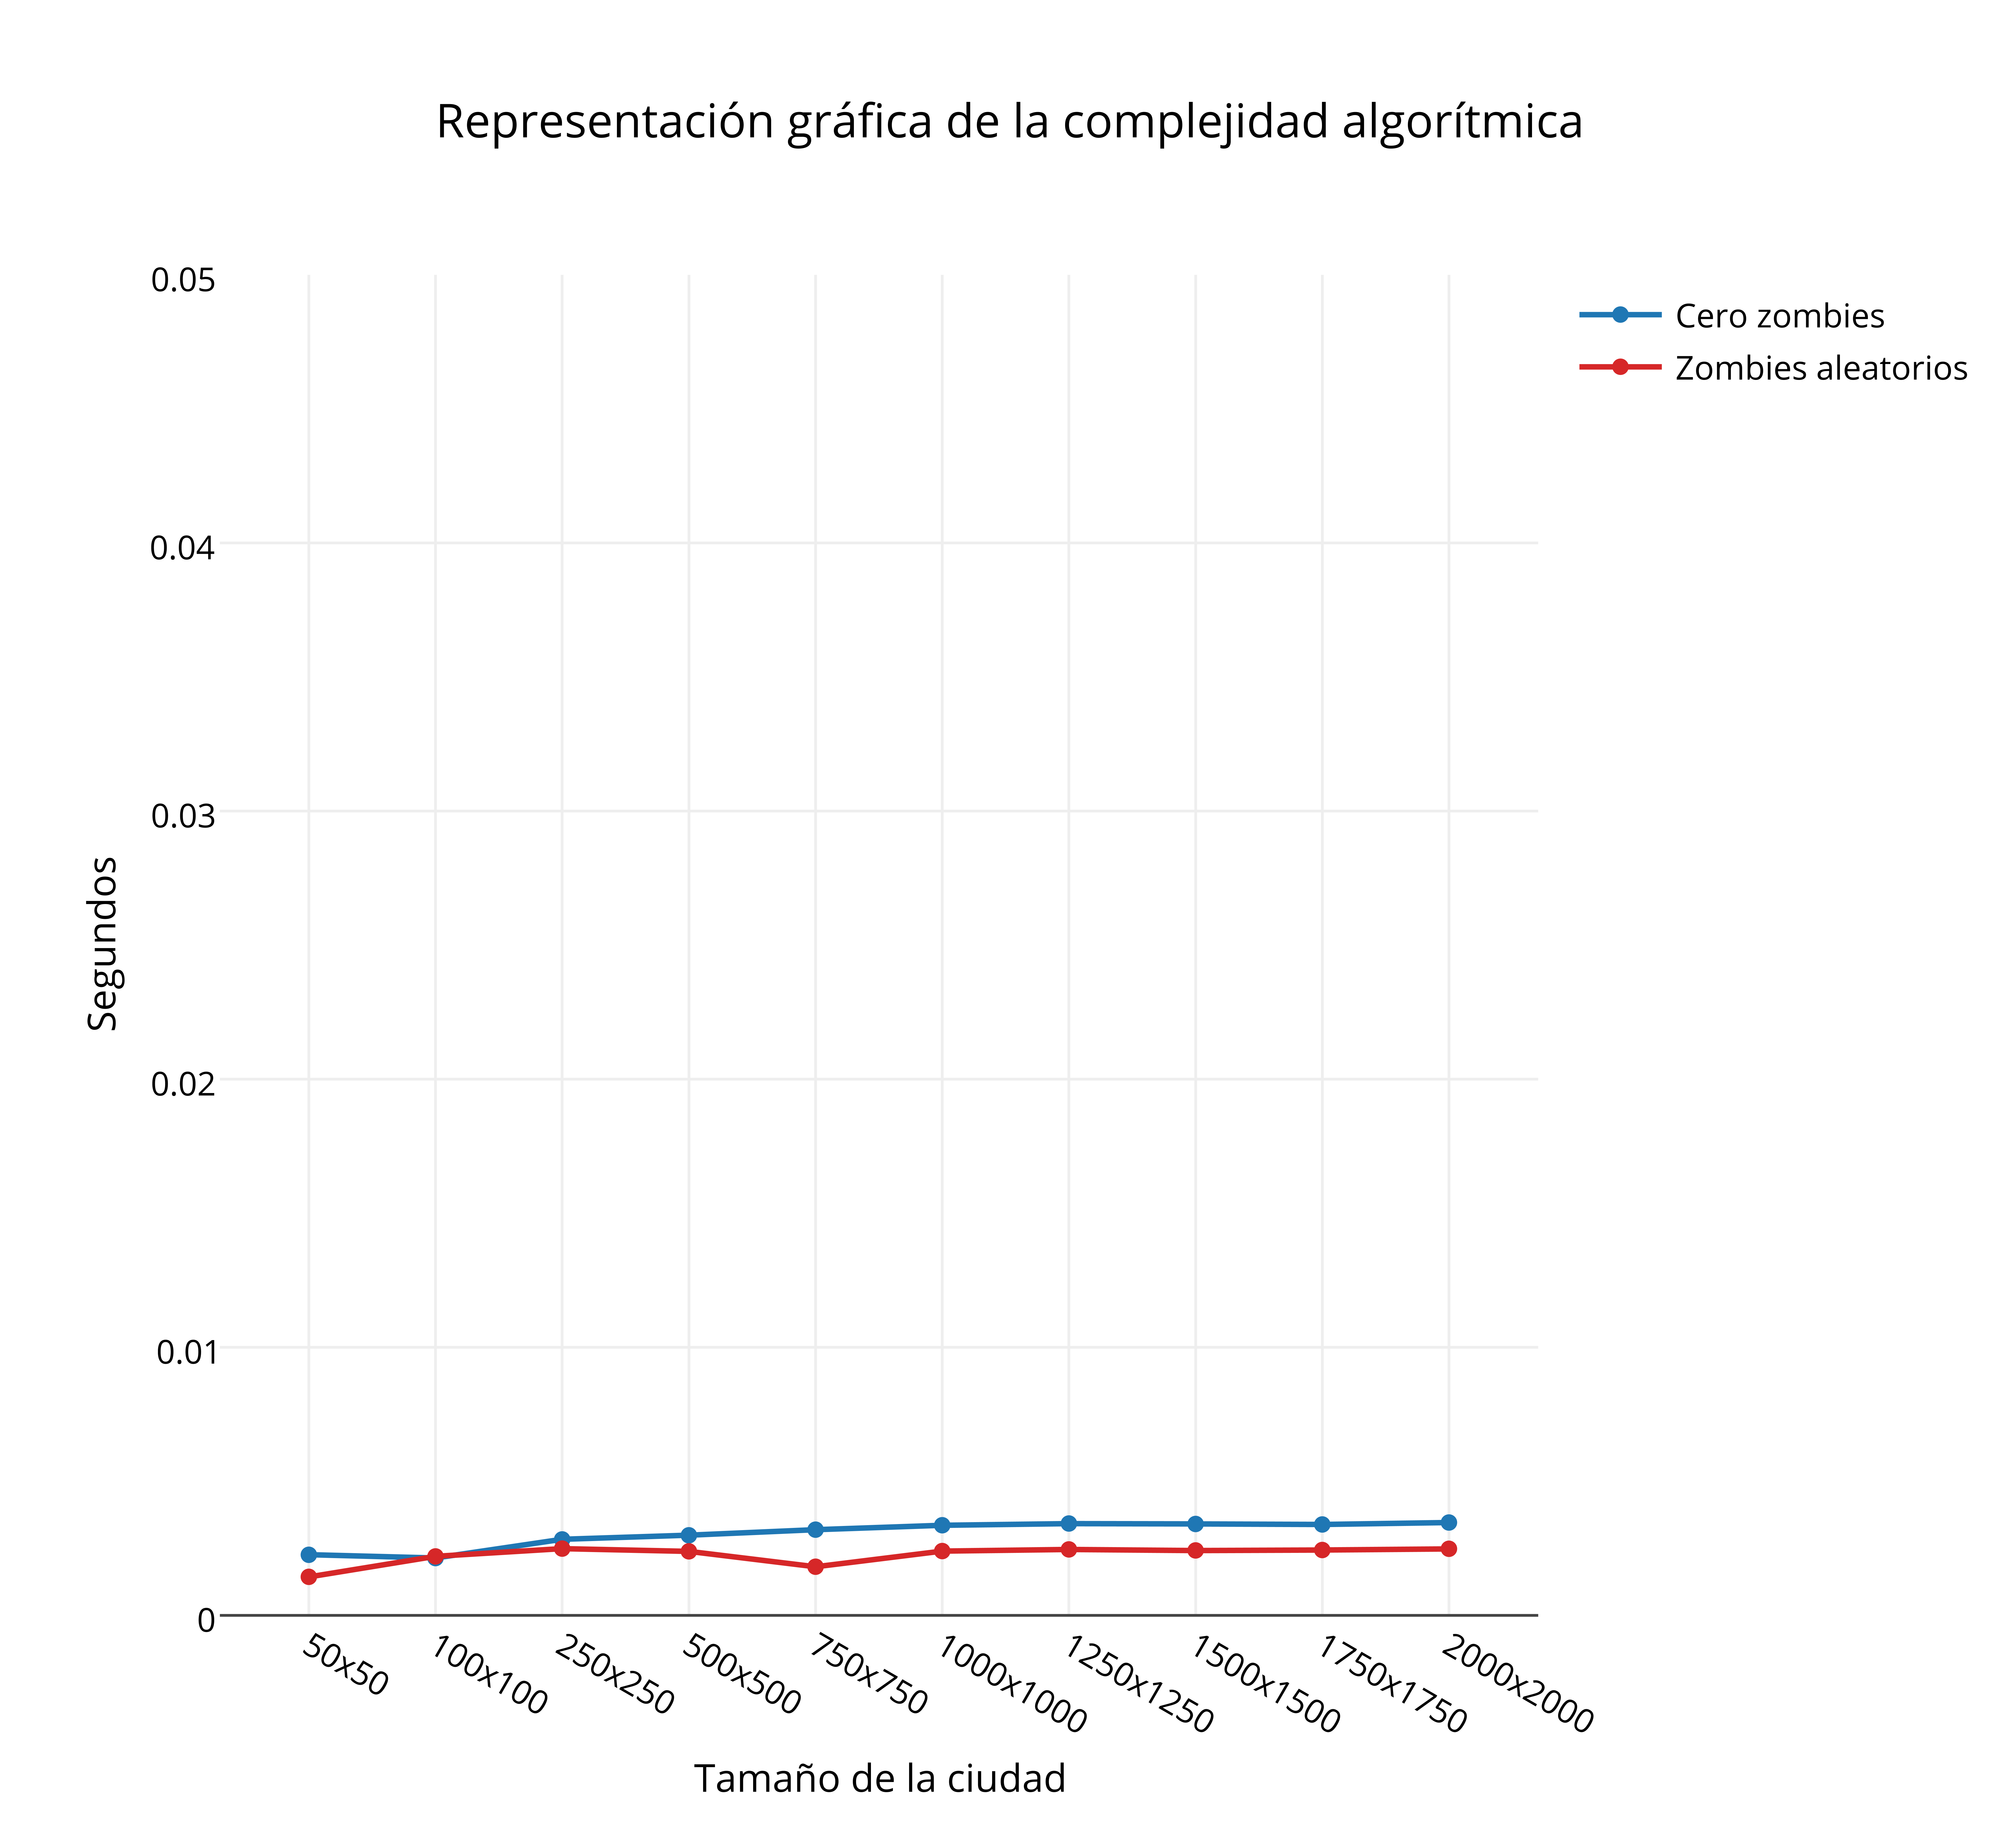
\includegraphics[width=15cm,keepaspectratio=yes]{imagenes/ej2/constantizacion.png}

Se puede ver que la experimentación se corresponde con la teoría, y que la complejidad, en peor caso, es $O(s.n.m)$.

